%
% THE BEER-WARE LICENSE (Rev. 42):
% Ronny Bergmann <bergmann@math.uni-luebeck.de> wrote this file. As long as you
% retain this notice you can do whatever you want with this stuff. If we meet
% some day, and you think this stuff is worth it, you can buy me a beer or
% coffee in return.
%
% This file is just to get started - You need the corresponding Logo
%
\documentclass[ngerman,10pt,xcolor=colortbl,compress
%,draft
]{beamer}
\usepackage{calc}
\usepackage[ngerman]{babel} % Neue Rechtschreibung
\usepackage{amsmath,amsthm,amssymb,euscript} % AMS-LaTeX  
\usepackage{enumerate,graphicx}
\usepackage{tikz}
%\usepackage[utf8]{inputenc}
\usepackage{fontspec}
\usepackage{pdfpages}
\usepackage{listings}
\usepackage{cmap}



% Load Them
\usetheme[slogan=false, navigation=true,reducedframetotal, myriad=false]{UzL}
%
\setbeamertemplate{navigation symbols}{}
\title{Bachelorprojekt }
\subtitle{Optimierung biologisch-realistischer Neuronenmodelle}
\date[]{14. Juli 2015\\[1ex]Abschlusspräsentation}
\author[Bereziak \and Dannehl \and Girth \and Kalelioglu \and Wolff]{S. Bereziak \and M. Dannehl \and C. Girth \and C. Kalelioglu \and J. Wolff}
% Clear Logo 1 to make the head smaller
\institute[UzL]{Institut für Robotik und kognitive Systeme\\Universität zu Lübeck}
%\clearlogo{1}
\setlogo{1}{.25\paperwidth}{logos/unilogo300dpi.png}%

\begin{document}

\defverbatim[colored]\makeset{%
	\begin{lstlisting}[ basicstyle=\tiny,  ]
	-----------------------------------------
	----------Welcome to opt_neuron----------
	-----------------------------------------
	For informations about the authors use the flag --version
	
	Executing commands from config...
	
	Welcome to the default Command Line Interface. You may enter a command now, e.g. "echo MESSAGE"
	To exit the program, type "exit" or on Unix hit Ctrl-D
	For a list of possible commands type "help"
	
	
	
	>get algorithms simple_genetic
	
	simple_genetic i_length p_count=100 generations=100 i_min=0 i_max=100 
	>
	\end{lstlisting}
}


	\maketitle
	\begin{frame}{Gliederung}
		\tableofcontents
	\end{frame}	
	
	\section{Überblick}
	\begin{frame}{Überblick}{Motivation}
	\begin{itemize}
	\item Parameter von neuronalen Netzen müssen stets optimiert werden
	\item Optimierungen von Hand sind sehr aufwendig bzw. praktisch unmöglich
	\end{itemize}
	\mbox{}\\
	$\rightarrow$ Automatisierte Optimierung mittels Methoden der künstlichen Intelligenz
	\end{frame}
	\begin{frame}{Überblick}{Zielsetzung}
	Framework, bestehend aus
	\begin{itemize}
		\item Strukturen zur Kommunikation mit neuronalem Netz
		\item Flexibel implementierte Optimierungsalgorithmen
		\item Grafische Oberfläche
	\end{itemize}
	\mbox{}\\
	Weitere Projektvorgaben
	\begin{itemize}
		\item Implementierung in Python
		\item Versionskontrolle über github
	\end{itemize}
	\end{frame}
	
	\section{Implementierung}
	
	\begin{frame}{Implementierung}{Struktur}
    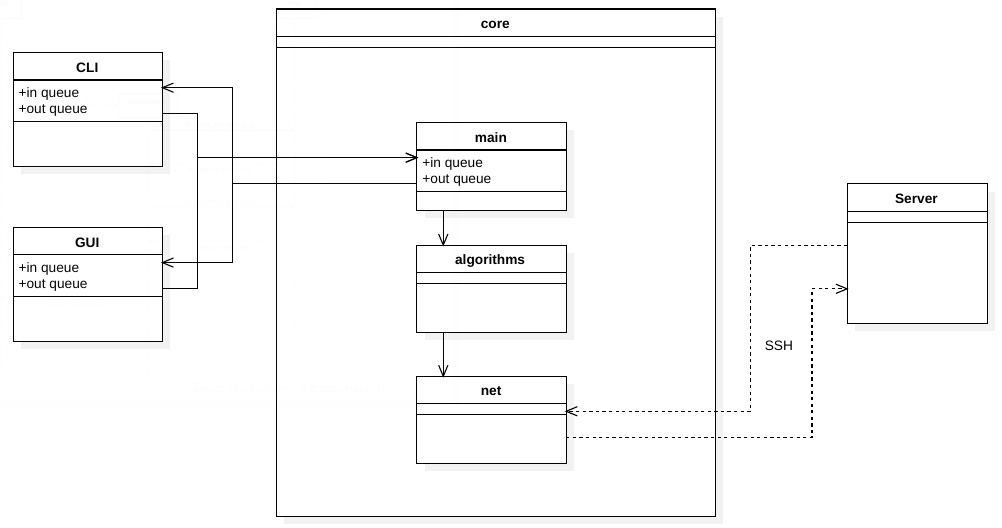
\includegraphics[scale=0.3]{module.png}
	\end{frame}
	\begin{frame}{Implementierung}{Kern}
	Der Kern besteht aus folgenden Komponenten
	\begin{itemize}
		\item main -- Verarbeitet Befehle von GUI oder CLI
		\item net -- Führt über SSH Netz und Analysescript aus
		\item algorithms -- Stellt Optimierungsalgorithmen bereit 
	\end{itemize}
	\mbox{}\\
	Kommunikation mit CLI bzw. GUI erfolgt über Message-Queues
	\end{frame}
	
	\begin{frame}
	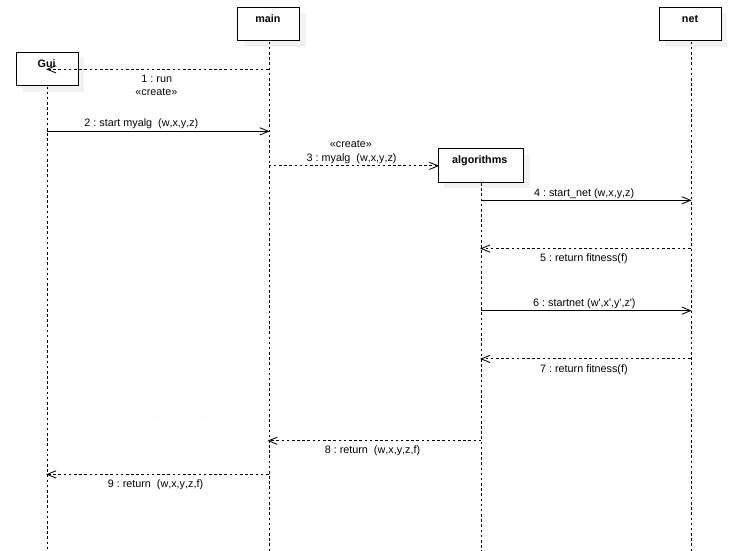
\includegraphics[scale=0.4]{sequenz.png}
	\end{frame}
	
	\begin{frame}{Implementierung}{Kern -- Implementierte Algorithmen}
	In der aktuellen Version implementierte Algorithmen
	\begin{itemize}
		\item simple\_genetic -- einfacher genetischer Algorithmus
		\item genetic2 -- weiterer genetischer Algorithmus
		\item random\_search -- randomisierte Suche
	\end{itemize}
	\end{frame}
	
	\begin{frame}{Implementierung}{CLI}
	\makeset
	\end{frame}

	\begin{frame}{Implementierung}{GUI}
	Die GUI besteht aus folgenden Gtk.Windows:
	\begin{itemize}
		\item mainframe -- Laden der Algorithmen und Starten/Speichern der Optimierung
		\item addframe -- Auswahl der Algorithmen und Setzen der Parameter
		\item sshframe -- Eingabe der SSH-Schlüsseldaten
	\end{itemize}
	\end{frame}
	
	\begin{frame}
	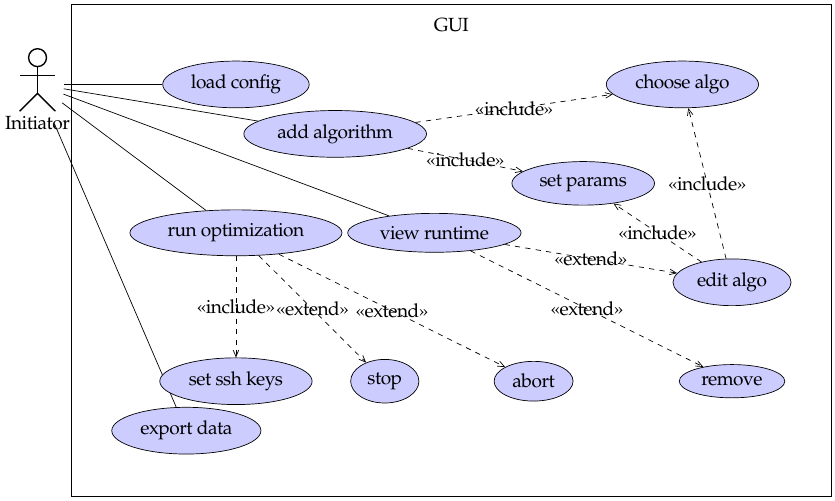
\includegraphics[scale=0.2]{GUI-use-case.png} 
	\end{frame}
	
	\begin{frame}{Implementierung}{Abhängigkeiten}
		Zur Ausführung benötigte Pakete
		\begin{itemize}
			\item python3
			\item sshpass
			\item GTK
			\item GDK
		\end{itemize}
	\end{frame}
	
	\section{Resultat}
	\begin{frame}{Resultat}{Live-Demo}
	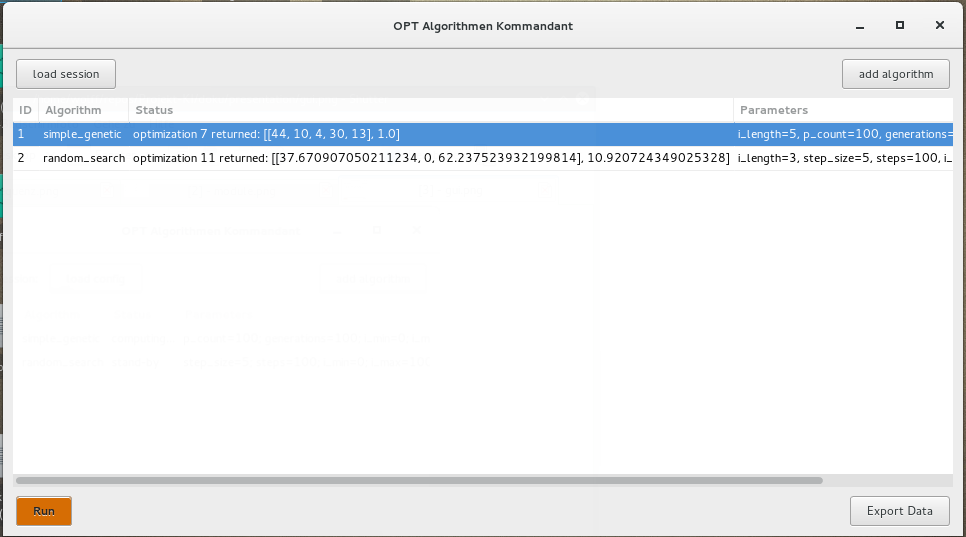
\includegraphics[scale=0.3]{gui.png}
	\end{frame}

	
\end{document}
